\pdfminorversion=7
\documentclass[tikz]{standalone}
\usetikzlibrary{arrows, calc, fit, hobby, positioning}
\pdfsuppresswarningpagegroup=1
\begin{document}
\newenvironment{localto}[2][]{
 \path let \p1=(#2.center), \p2=(#2.north), \p3=(#2.east) in coordinate (#2X) at (\x3-\x1,0) coordinate (#2Y) at (0,\y2-\y1);
 \begin{scope}[x={(#2X)}, y={(#2Y)}, shift={(#2.center)},#1]
}{
 \end{scope}
}
\newcommand\stepnode[3][]{
 \node (#2_lbl) [#1] {#2};
 \node (#2_pts) [below=0 of #2_lbl, draw, minimum width=1cm, minimum height=.5cm] {};
 \node (#2) [fit=(#2_lbl)(#2_pts)] {};
 \begin{localto}{#2_pts}
 \foreach \i in {0,...,100} {
  \pgfmathsetmacro{\x}{.9 * (2*rnd-1)}
  \pgfmathsetmacro{\y}{.9 * (2*rnd-1)};
  \fill [gray] (\x, \y) circle (.01cm);
 }
 \node (#2_pt) at (#3) [draw=red, circle, inner sep=0pt, minimum size=.01cm] {};
 \end{localto}
}
\begin{tikzpicture}[>=stealth']
 \stepnode{Init}{0, -.9};
 \stepnode[above left=of Init]{Develop}{-.9, 0};
 \node[above right=of Develop] (Evaluate) {Evaluate};
 \node[below right=of Evaluate] (Mutate) {Mutate};

 \draw [->] (Init) to [out=180, in=270] (Develop);
 \draw [->] (Develop) to [out=90, in=180] (Evaluate);
 \draw [->] (Evaluate) to [out=0, in=90] (Mutate);
 \draw [->] (Evaluate) to [out=300, in=240, looseness=6] node [pos=.5, anchor=north] {Learn} (Evaluate);
 \draw [->] (Mutate) to [out=270, in=0] (Develop);

 % --

 \node (Init_details) [below=of Init, inner sep=0pt] {};
 \node (body_genome) [below left=0 of Init_details]
  {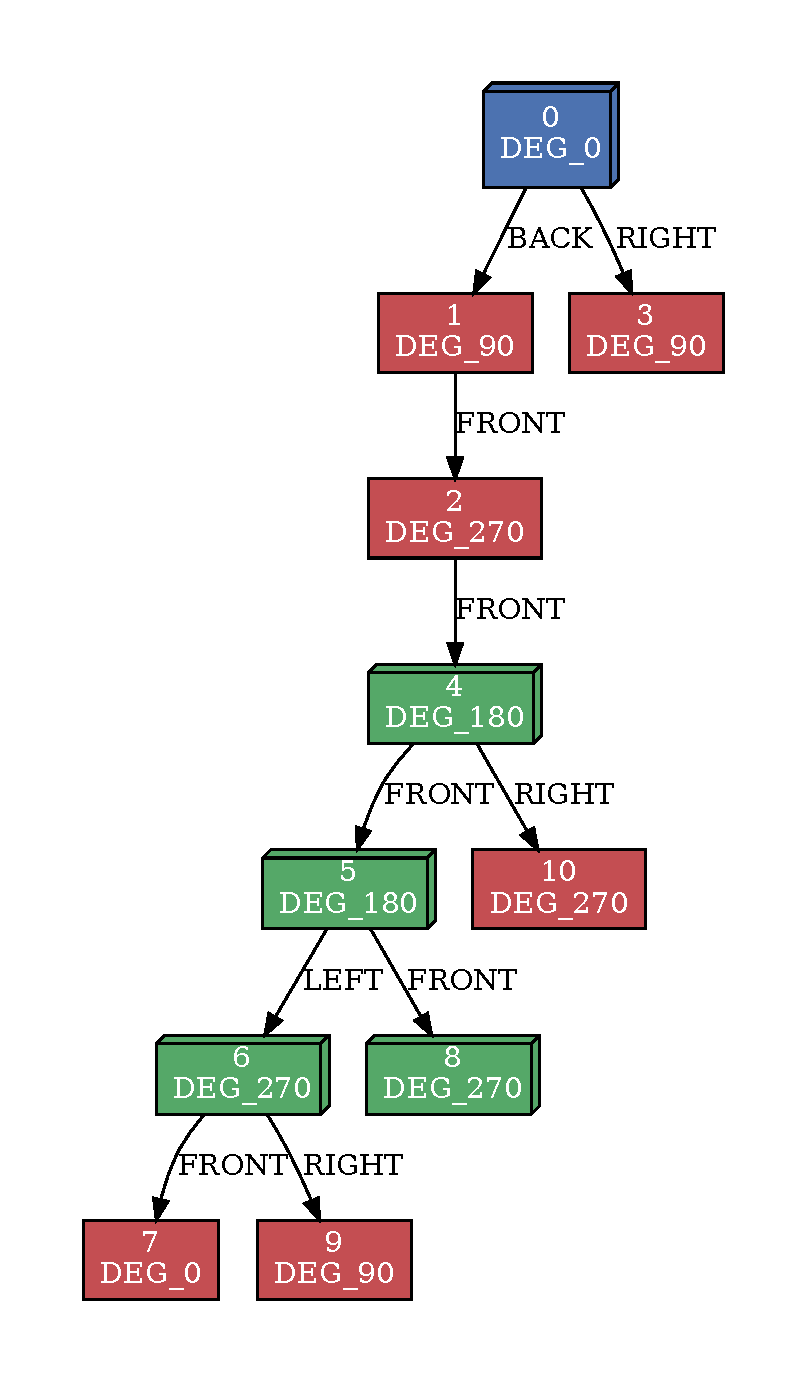
\includegraphics[width=.75cm, angle=90]{genome_body}};
 \node [above=0 of body_genome, font=\tiny, scale=.75] {\emph{Morphology}};
 \node (brain_genome) [below right=0 of Init_details]
  {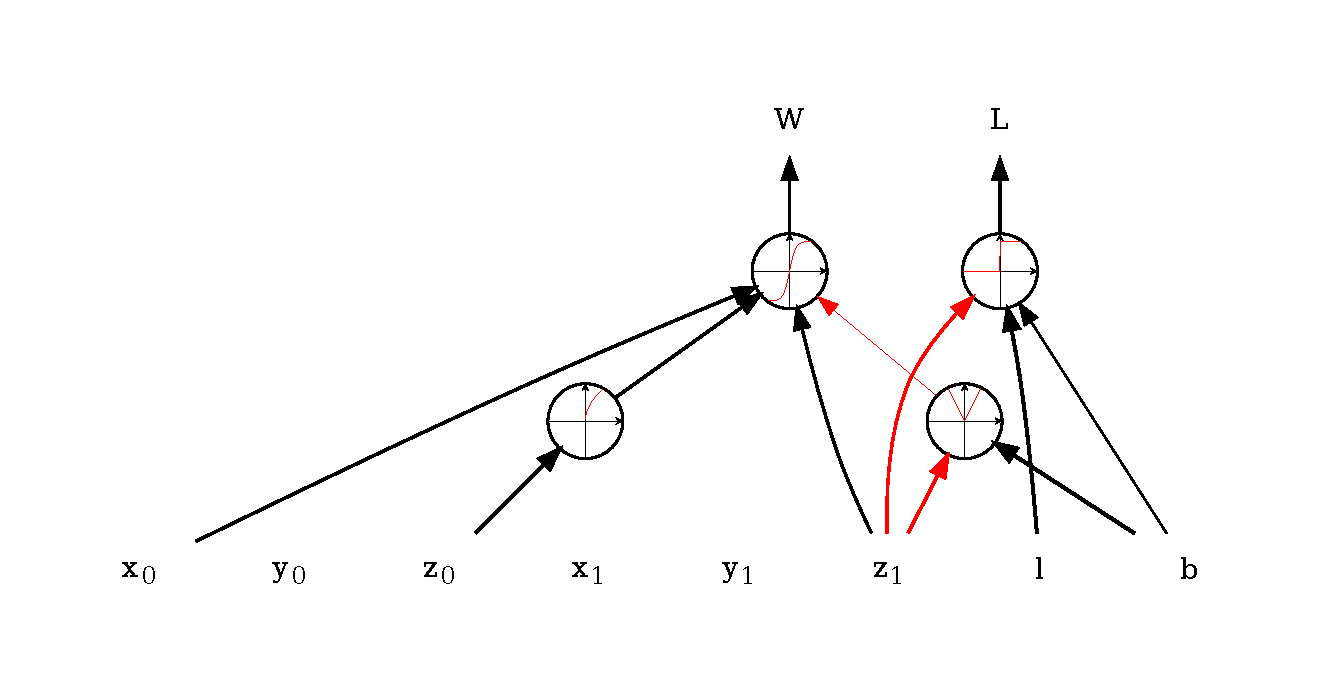
\includegraphics[height=.75cm]{genome_brain}};
 \node (brain_genome_label) [above=0 of brain_genome, font=\tiny, scale=.75] {\emph{Controller}};
 \node (Init_inset) [fit=(body_genome)(brain_genome_label)(brain_genome), draw] {};
 \node at (Init_inset.south) [anchor=south, font=\tiny, inner sep=1pt] {Genotypes};
 \draw [dotted, gray] (Init_inset.north west) -- (Init_pt.west)
                      (Init_inset.north east) -- (Init_pt.east);

 % --

 \node (Develop_details) [left=of Develop, inner sep=0pt] {};
 \node (body) [above=.125 of Develop_details, inner sep=0pt]
  {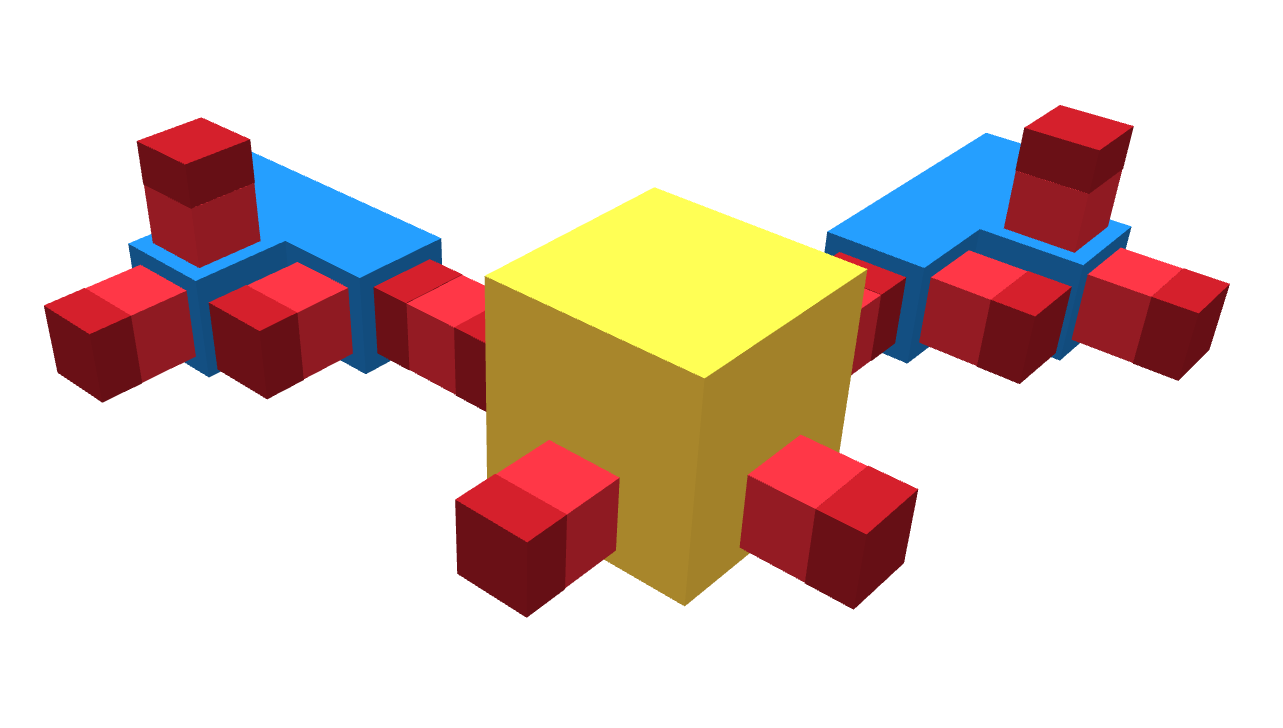
\includegraphics[width=1cm]{../elb6/snail}};
 \node (body_label) [above=0 of body, font=\tiny, scale=.75] {\emph{Morphology}};
 \node (brain) [below=.125 of Develop_details, inner sep=0pt]
  {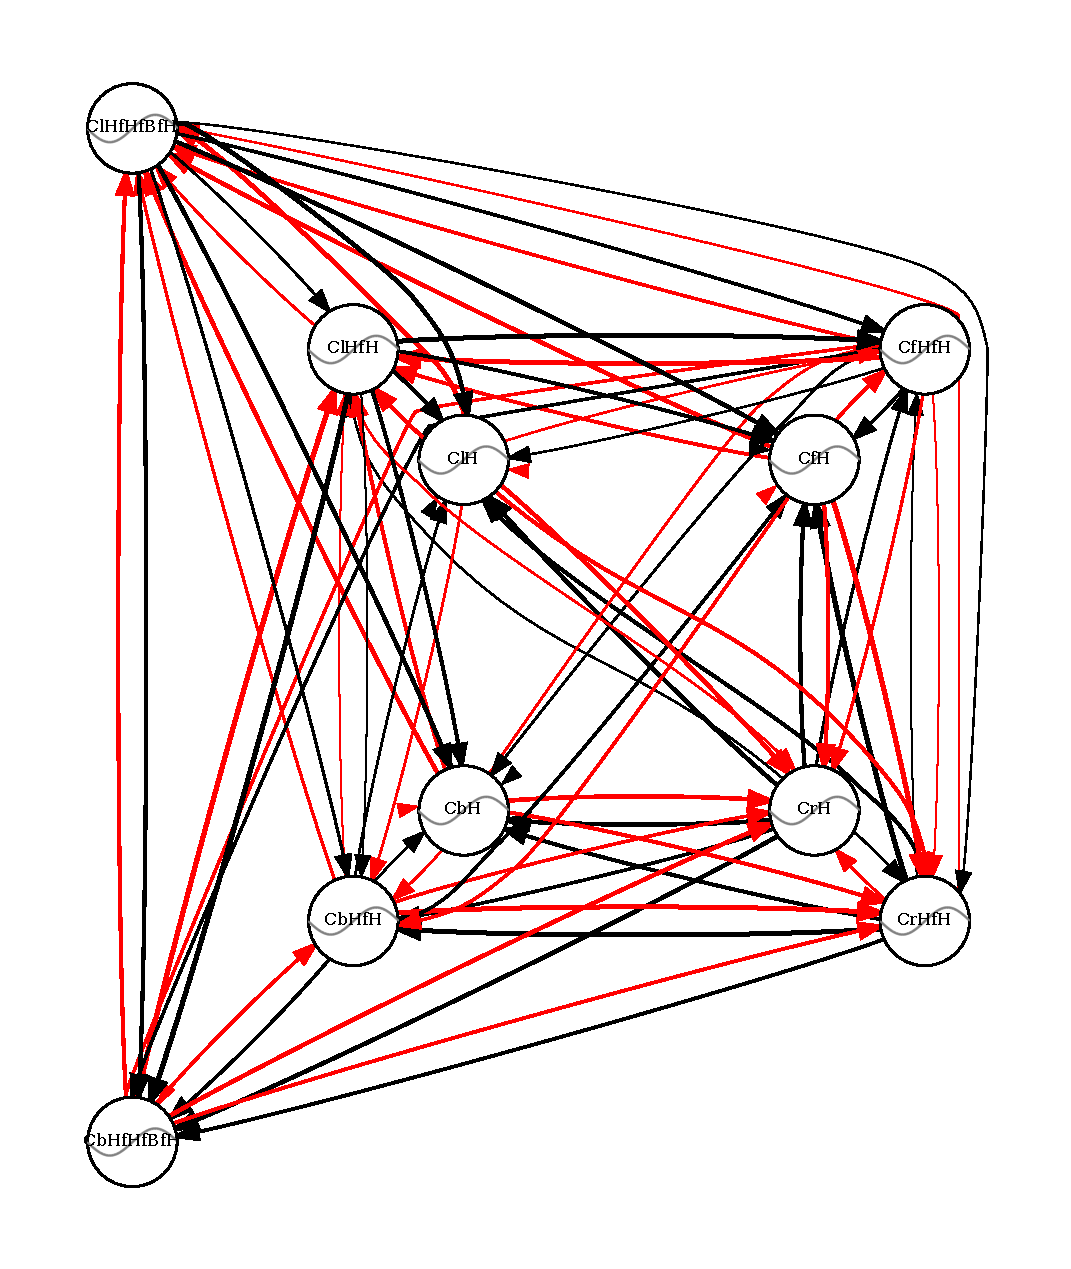
\includegraphics[width=1cm]{brain}};
 \node (brain_label) [above=0 of brain, font=\tiny, scale=.75] {\emph{Controller}};
 \node (phenotype_margin) [below=0 of brain] {};
 \node (Develop_inset) [fit=(body_label)(brain)(phenotype_margin), draw] {};
 \node at (Develop_inset.south) [anchor=south, font=\tiny, inner sep=1pt] {Phenotypes};
 \draw [dotted, gray] (Develop_inset.north east) -- (Develop_pt.north)
                      (Develop_inset.south east) -- (Develop_pt.south);

 % --

 \node (Evaluate_details) [above=0 of Evaluate, inner sep=0pt] {};
 \node (task) [above=0 of Evaluate_details, inner sep=0pt]
  {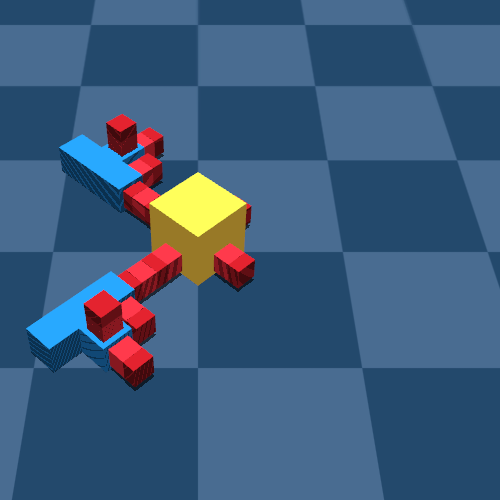
\includegraphics[width=1cm]{task}};
 \draw [->, green!60!white, thick] (task.center) ++(.05, 0) -- ++(.3, 0);

 % =====
 % Eval

 \node [draw] (CPG_r) at (6, 0) {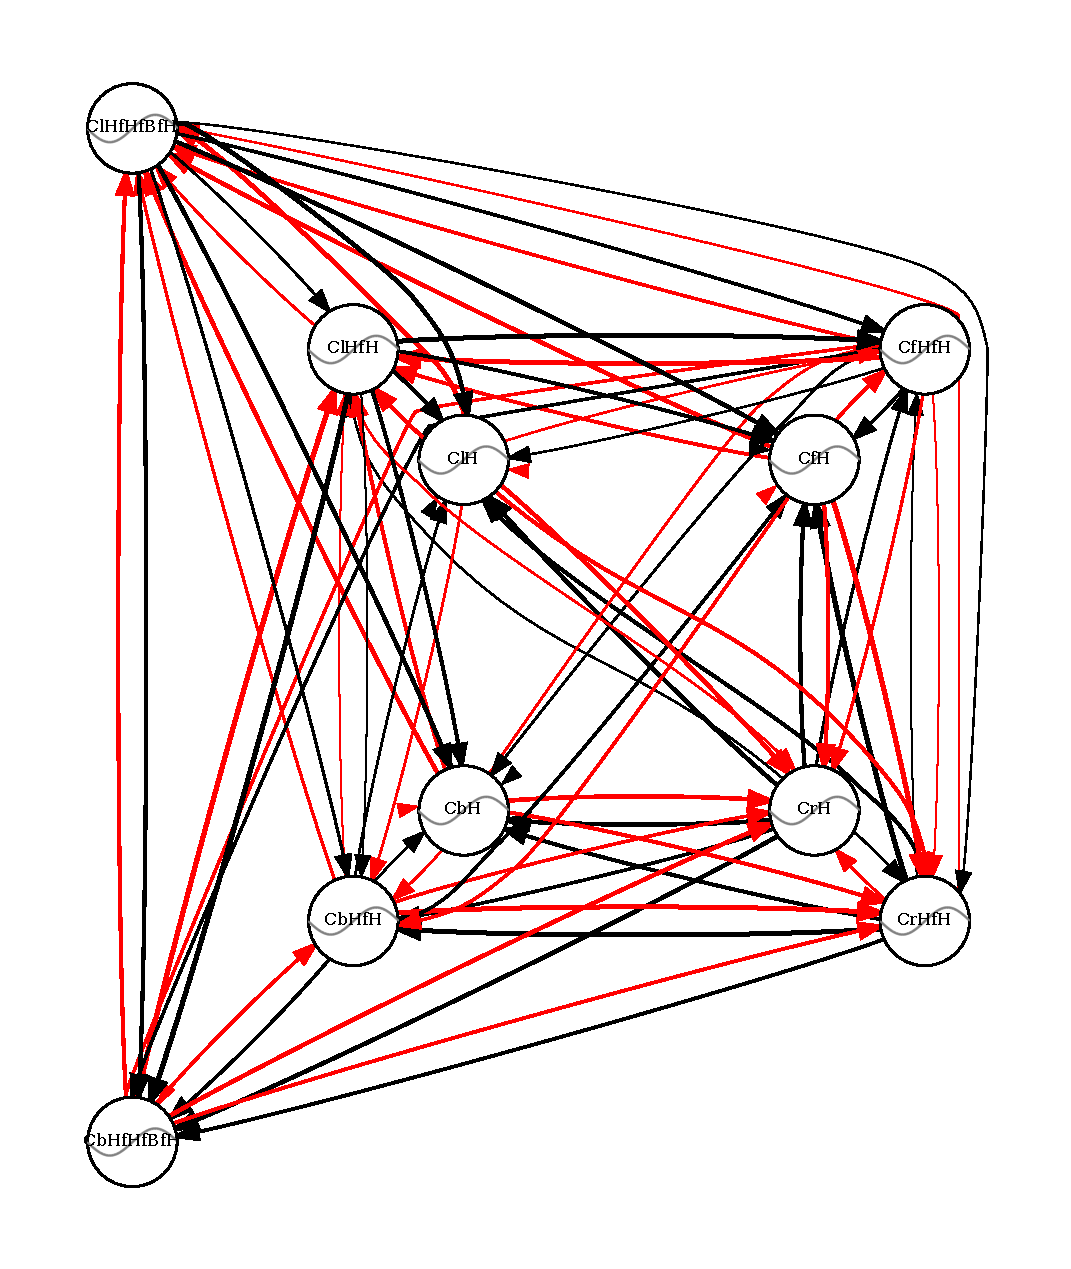
\includegraphics[width=1cm]{brain}};
 \node at (CPG_r) [fill=white, fill opacity=.5, text opacity=1] {CPG};
 \node [above=0 of CPG_r] (abCPG) {$\alpha\beta-$CPG};
 \node (abcpg_all) [fit=(CPG_r)(abCPG), draw] {};
 \foreach \i in {4,...,0} {
  \node [draw, above=0 of abCPG, shift={(.1*\i,.1*\i)}, fill=white] (policy_\i) {Policy};
  \node [draw, right=of abCPG, shift={(.1*\i,.1*\i)}, fill=white] (env_\i) {Environment};

  \def\envs{{"fetch", "carrying", "obstacles", "parking", "+figure8"}}
  \node [below=0 of env_\i, inner sep=0pt, draw, ultra thick]
   {\pgfmathparse{\envs[\i]}\includegraphics[width=1cm]{../tasks/\pgfmathresult}};
 }

 \draw [->] (Evaluate) -- ++(2.5, 0)
  to [out=0, in=180, looseness=1.5]
  node [pos=0.5] (transfer) {}
  (CPG_r);

 \coordinate (t) at ($(transfer.base)+(-.3ex, 0)$);
 \draw [dotted] (t |- current bounding box.south) -- (t |- current bounding box.north)
  coordinate (top);

 \node at (transfer) [rotate=-90, fill=white] {\textbf{Transfer}};
 \node [below left=0 of top, anchor=north east] {\textbf{Training}};
 \node [below right=0 of top, anchor=north west] {\textbf{Deployment}};
\end{tikzpicture}
\end{document}
